\subsubsection{Datasets and Cuts}
In this Run11 $D^0$ re-analysis, we ran 461 million events ($\sim$85\% of total). Cuts are listed in the following.
\begin{itemize}
\item \textbf{Library}: P11id.

\item \textbf{Trigger IDs}:  350003, 350013, 350023, 350033, 350043.

\item \textbf{Centrality}: 0-80\%.

\item \textbf{Vertex selections}
\begin{itemize}
\item $|v_z^{TPC}| < 30$ cm
\item $|v_z^{TPC} - v_z^{VPD}| < 3$ cm
\end{itemize}

\item \textbf{Track selections}
\begin{itemize}
\item $p_T > 0.2$ GeV/c
\item $|\eta| < 1$
\item $\mathrm{global ~ DCA} < 1$ cm
\item $20 \leq \mathrm{nHitsFit} < 50$
\item $\mathrm{nHitsFit}/\mathrm{nHitsMax} > 0.52$
\item $\mathrm{nHitsdEdx} > 10$
\end{itemize}

\item \textbf{PID}
\begin{itemize}
\item TPC PID (dE/dx): $|n\sigma_K| < 2$ and $|n\sigma_\pi| < 3$
\item TOF PID (1/$\beta$): define $n\sigma_X^{TOF} = ( \frac{1}{\beta} - \sqrt{m_X^2/p^2 + 1} )/\sigma + c$, here $\sigma = 0.013$, $c = 0.3$,  $m_X$ is particle ($K$, $\pi$, etc.) mass. For pions, we apply $n\sigma_\pi^{TOF} < f_\pi^{\mathrm{max}}(p)$, here
\begin{equation}
f_\pi^{\mathrm{max}}(p) = \left\{
\begin{aligned}
&5.43 - 2.14x, ~ p < 1.6  \\
&2, ~ p \geq 1.6
\end{aligned}
\right.
\label{eq:nsigTofPi}
\end{equation}
For kaons, we apply $f_K^{\mathrm{min}}(p) < n\sigma_K^{TOF} < f_K^{\mathrm{max}}(p)$, here
\begin{equation}
f_K^{\mathrm{min}}(p) = \left\{
\begin{aligned}
&-7.54 + 5.83p - 1.31p^2, ~ p < 1.3  \\
&-2, ~ p \geq 1.3
\end{aligned}
\right.
\label{eq:nsigTofK1}
\end{equation}

\begin{equation}
f_K^{\mathrm{max}}(p) = \left\{
\begin{aligned}
&8.69 - 6.02p + 1.32p^2, ~ p < 2.0  \\
&2, ~ p \geq 2.0
\end{aligned}
\right.
\label{eq:nsigTofK1}
\end{equation}

There are two PID cases:
\begin{itemize}
\item hybrid PID: Apply TOF PID while TOF is available (TOFMatchFlag $>$ 0 \&\& $\beta > 0$  \&\& pathLength $>$ 200 \&\& $|\mathrm{ylocal}| < 1.8$) , otherwise use TPC PID only.
\item clean PID: It's the same as hybrid PID, except that TOF match must be required at $p < 1.6$ GeV/c (TOFMatchFlag $>$ 0). 
\end{itemize}
\end{itemize}

\item \textbf{$D^0$ rapidity}: $|y| < 1$
\end{itemize}

\subsubsection{$D^0$ recronstruction}
We reconstruct $D^0$ through the channel $D^0 \rightarrow K^-\pi^+$(B.R. = 0.0388). Background is reconstructed with mix-event method. 9 centrality bins (0-80\%) and 10 primary vertex $v_z$ bins ($v_z \in [-30,30]$ cm) are used to classify mixed events with some degree of similarity. Mix-event unlike-sign background is scaled to same-event like-sign background at the mass region of $1.69 < \mathrm{mass}_{K\pi} < 2.04$ GeV/$c^2$. Then same event unlike-sign (signal + background) subtracted by scaled mix-event unlike-sign background are fitted with a gaussian function (signal) plus a second order polynomial function (residual background). The fit range is 1.69-2.04 GeV/$c^2$.

Fig.~\ref{fig:Run11TpcClean0_80} shows $D^0$ signal at 6 $p_T$ bins (0-0.7, 0.7-1.1, 1.1-1.6, 1.6-2.2, 2.2-3.0, 3.0-5.0) in 0-80\% with clean PID.
\begin{figure}
    \centering
    \subfigure{\includegraphics[width=0.32\textwidth]{{figure/Run11_xiaolong/ptDivision1/cleanPID/cent0_80_pt_0.0_0.7}.eps}}
    \subfigure{\includegraphics[width=0.32\textwidth]{{figure/Run11_xiaolong/ptDivision1/cleanPID/cent0_80_pt_0.7_1.1}.eps}}
    \subfigure{\includegraphics[width=0.32\textwidth]{{figure/Run11_xiaolong/ptDivision1/cleanPID/cent0_80_pt_1.1_1.6}.eps}} \\
    \subfigure{\includegraphics[width=0.32\textwidth]{{figure/Run11_xiaolong/ptDivision1/cleanPID/cent0_80_pt_1.6_2.2}.eps}} 
    \subfigure{\includegraphics[width=0.32\textwidth]{{figure/Run11_xiaolong/ptDivision1/cleanPID/cent0_80_pt_2.2_3.0}.eps}}
    \subfigure{\includegraphics[width=0.32\textwidth]{{figure/Run11_xiaolong/ptDivision1/cleanPID/cent0_80_pt_3.0_5.0}.eps}}
    \caption{$D^0$ signal at 6 $p_T$ bins (0-0.7, 0.7-1.1, 1.1-1.6, 1.6-2.2, 2.2-3.0, 3.0-5.0) in 0-80\% with clean PID.}
   \label{fig:Run11TpcClean0_80}
\end{figure}

Fig.~\ref{fig:Run11TpcHybrid0_80} shows $D^0$ signal at 6 $p_T$ bins (0-0.7, 0.7-1.1, 1.1-1.6, 1.6-2.2, 2.2-3.0, 3.0-5.0) in 0-80\% with hybrid PID.
\begin{figure}
    \centering
    \subfigure{\includegraphics[width=0.32\textwidth]{{figure/Run11_xiaolong/ptDivision1/hybridPID/cent0_80_pt_0.0_0.7}.eps}}
    \subfigure{\includegraphics[width=0.32\textwidth]{{figure/Run11_xiaolong/ptDivision1/hybridPID/cent0_80_pt_0.7_1.1}.eps}}
    \subfigure{\includegraphics[width=0.32\textwidth]{{figure/Run11_xiaolong/ptDivision1/hybridPID/cent0_80_pt_1.1_1.6}.eps}} \\
    \subfigure{\includegraphics[width=0.32\textwidth]{{figure/Run11_xiaolong/ptDivision1/hybridPID/cent0_80_pt_1.6_2.2}.eps}} 
    \subfigure{\includegraphics[width=0.32\textwidth]{{figure/Run11_xiaolong/ptDivision1/hybridPID/cent0_80_pt_2.2_3.0}.eps}}
    \subfigure{\includegraphics[width=0.32\textwidth]{{figure/Run11_xiaolong/ptDivision1/hybridPID/cent0_80_pt_3.0_5.0}.eps}}
    \caption{$D^0$ signal at 6 $p_T$ bins (0-0.7, 0.7-1.1, 1.1-1.6, 1.6-2.2, 2.2-3.0, 3.0-5.0) in 0-80\% with hybrid PID.}
   \label{fig:Run11TpcHybrid0_80}
\end{figure}

Fig.~\ref{fig:Run11TpcClean} shows $D^0$ signal at 2 $p_T$ bins (0-2, 2-4) and 4 centralilties (0-80\%, 0-10\%, 10-40\%, 40-80\%) with clean PID.
\begin{figure}
    \centering
    \subfigure{\includegraphics[width=0.32\textwidth]{{figure/Run11_xiaolong/cleanPID/cent0_80_pt_0.0_2.0}.eps}}
    \subfigure{\includegraphics[width=0.32\textwidth]{{figure/Run11_xiaolong/cleanPID/cent0_80_pt_2.0_4.0}.eps}}
    \subfigure{\includegraphics[width=0.32\textwidth]{{figure/Run11_xiaolong/cleanPID/cent0_10_pt_0.0_2.0}.eps}}  \\
    \subfigure{\includegraphics[width=0.32\textwidth]{{figure/Run11_xiaolong/cleanPID/cent0_10_pt_2.0_4.0}.eps}} 
    \subfigure{\includegraphics[width=0.32\textwidth]{{figure/Run11_xiaolong/cleanPID/cent10_40_pt_0.0_2.0}.eps}}
    \subfigure{\includegraphics[width=0.32\textwidth]{{figure/Run11_xiaolong/cleanPID/cent10_40_pt_2.0_4.0}.eps}} \\
    \subfigure{\includegraphics[width=0.32\textwidth]{{figure/Run11_xiaolong/cleanPID/cent40_80_pt_0.0_2.0}.eps}}
    \subfigure{\includegraphics[width=0.32\textwidth]{{figure/Run11_xiaolong/cleanPID/cent40_80_pt_2.0_4.0}.eps}}
    \caption{$D^0$ signal at 2 $p_T$ bins (0-2, 2-4) and 4 centralilties (0-80\%, 0-10\%, 10-40\%, 40-80\%) with clean PID.}
   \label{fig:Run11TpcClean}
\end{figure}

Fig.~\ref{fig:Run11TpcHybrid} shows $D^0$ signal at 2 $p_T$ bins (0-2, 2-4) and 4 centralilties (0-80\%, 0-10\%, 10-40\%, 40-80\%) with hybrid PID.
\begin{figure}
    \centering
    \subfigure{\includegraphics[width=0.32\textwidth]{{figure/Run11_xiaolong/hybridPID/cent0_80_pt_0.0_2.0}.eps}}
    \subfigure{\includegraphics[width=0.32\textwidth]{{figure/Run11_xiaolong/hybridPID/cent0_80_pt_2.0_4.0}.eps}}
    \subfigure{\includegraphics[width=0.32\textwidth]{{figure/Run11_xiaolong/hybridPID/cent0_10_pt_0.0_2.0}.eps}}  \\
    \subfigure{\includegraphics[width=0.32\textwidth]{{figure/Run11_xiaolong/hybridPID/cent0_10_pt_2.0_4.0}.eps}} 
    \subfigure{\includegraphics[width=0.32\textwidth]{{figure/Run11_xiaolong/hybridPID/cent10_40_pt_0.0_2.0}.eps}}
    \subfigure{\includegraphics[width=0.32\textwidth]{{figure/Run11_xiaolong/hybridPID/cent10_40_pt_2.0_4.0}.eps}} \\
    \subfigure{\includegraphics[width=0.32\textwidth]{{figure/Run11_xiaolong/hybridPID/cent40_80_pt_0.0_2.0}.eps}}
    \subfigure{\includegraphics[width=0.32\textwidth]{{figure/Run11_xiaolong/hybridPID/cent40_80_pt_2.0_4.0}.eps}}
    \caption{$D^0$ signal at 2 $p_T$ bins (0-2, 2-4) and 4 centralilties (0-80\%, 0-10\%, 10-40\%, 40-80\%) with hybrid PID.}
   \label{fig:Run11TpcHybrid}
\end{figure}

\subsubsection{Efficiency and acceptance correction}
The efficiency and acceptance correction includes the following:
\begin{itemize}
\item Acceptance, including $p_T$ and $\eta$ cut efficiency.
\item TPC tracking efficiency, including the basic track quality cut efficiency. ndEdxHits cut efficiency is not included.
\item ndEdxHits cut efficency. This efficiency is obtained from data ( track number with ndEdxHits cut  divided by that without ndEdxHits cut ).
\item TOF matching efficiency.
\item PID efficiency, including TOF PID and TPC PID efficiency.
\end{itemize}

Among them, TPC tracking efficiency, PID efficiency is obtained from Yifei (published Run10+11 $D^0$).

Fig.~\ref{fig:Run11ndEdx} shows ndEdxHits cut efficiency. It's very high both for $K$ and $\pi$ ($\sim$ 99\%).
\begin{figure}
    \centering
    \subfigure{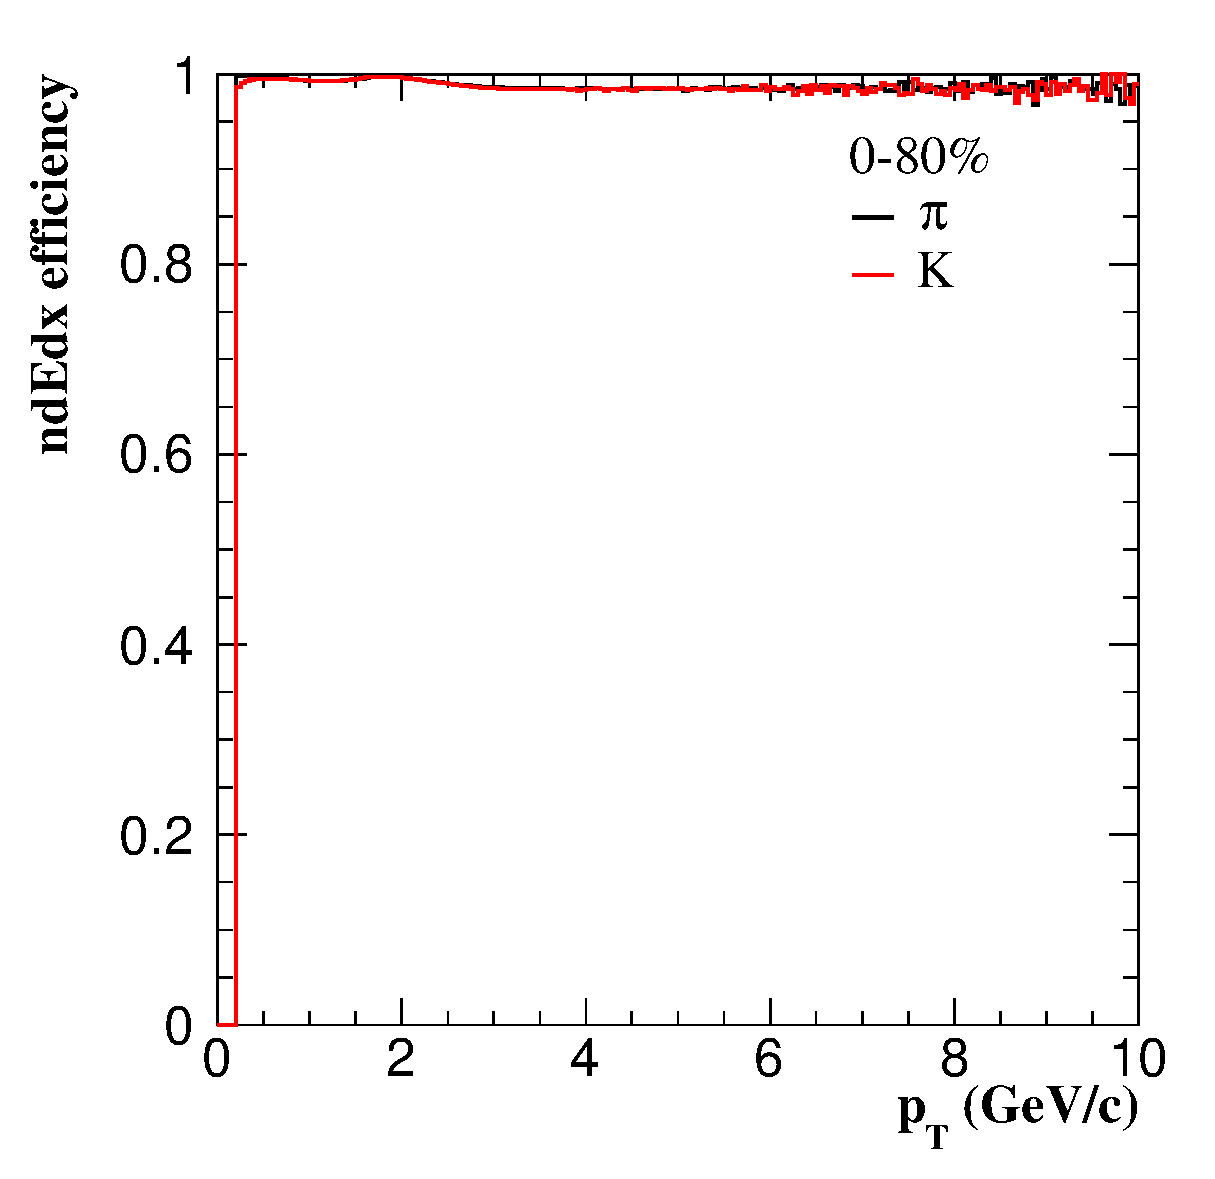
\includegraphics[width=0.5\textwidth]{{figure/Run11_xiaolong/efficiency/ndEdxEff}.eps}}
    \caption{Run11 ndEdxHits cut efficiency.}
   \label{fig:Run11ndEdx}
\end{figure}

Fig.~\ref{fig:Run11TofMatch} shows $K/\pi$ TOF matching efficiency at 0-80\%, 0-10\%, 10-40\%, 40-80\%. The dip at the $p_{T}$ region of 0.5-0.9 GeV/c for kaons is due that we use $n\sigma_{K/\pi}$ to identify $K/\pi$ and $n\sigma_K$ resolution get better at low $p_T$ when TOF match is required. Detailed validation can be found at Section~\ref{sec:TOFmatch}.
\begin{figure}
    \centering
    \subfigure{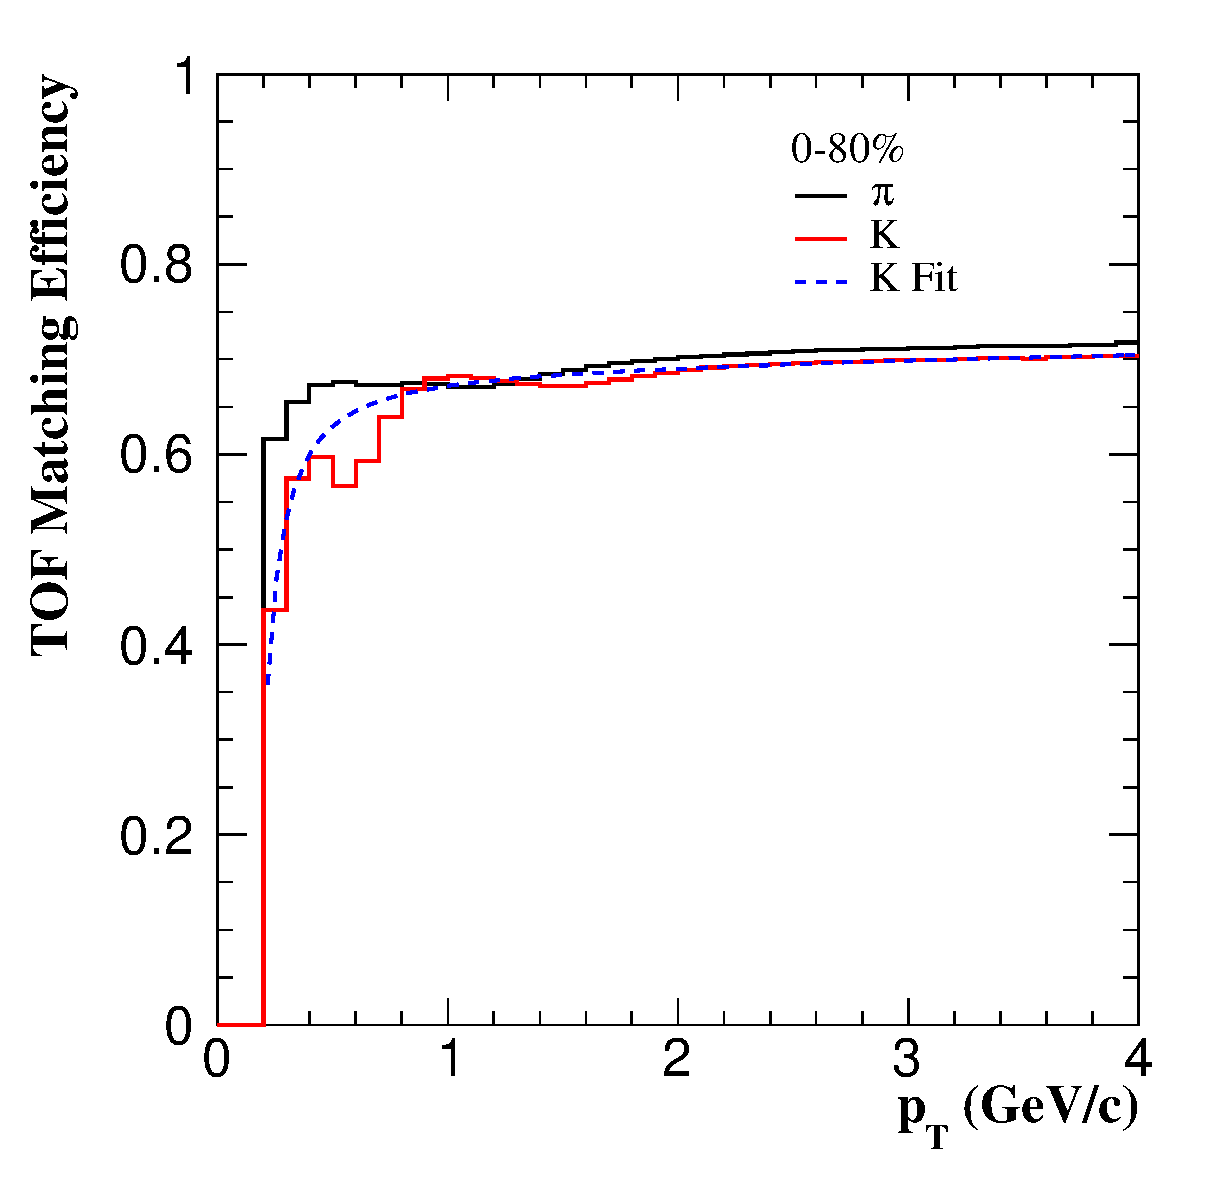
\includegraphics[width=0.47\textwidth]{{figure/Run11_xiaolong/efficiency/tofMatchRun11_0_80}.eps}}
    \subfigure{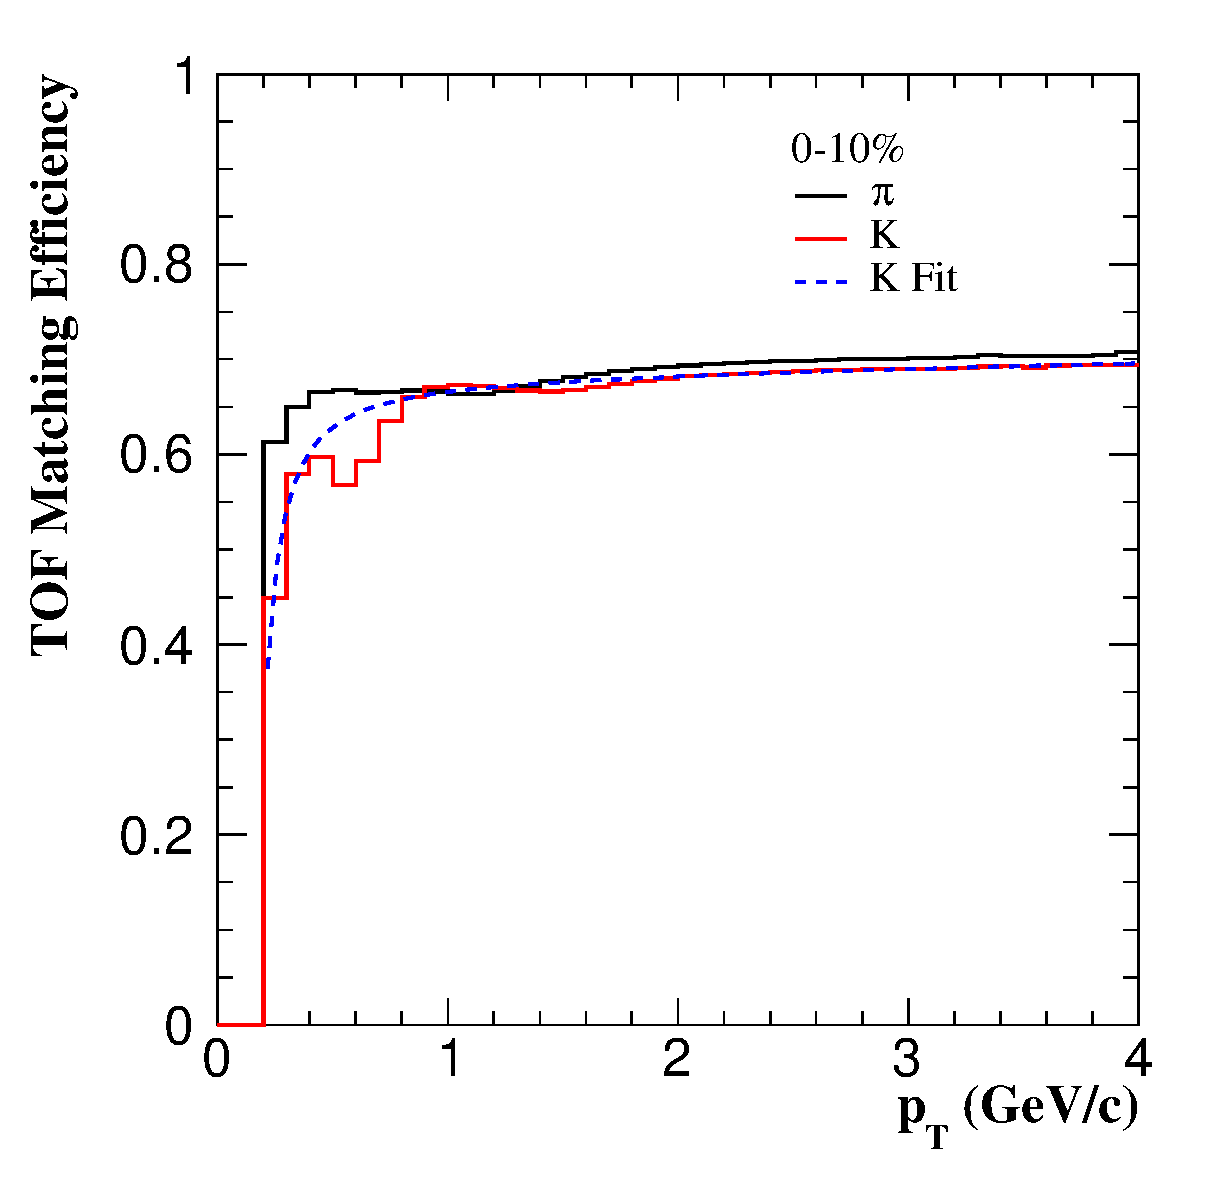
\includegraphics[width=0.47\textwidth]{{figure/Run11_xiaolong/efficiency/tofMatchRun11_0_10}.eps}} \\
    \subfigure{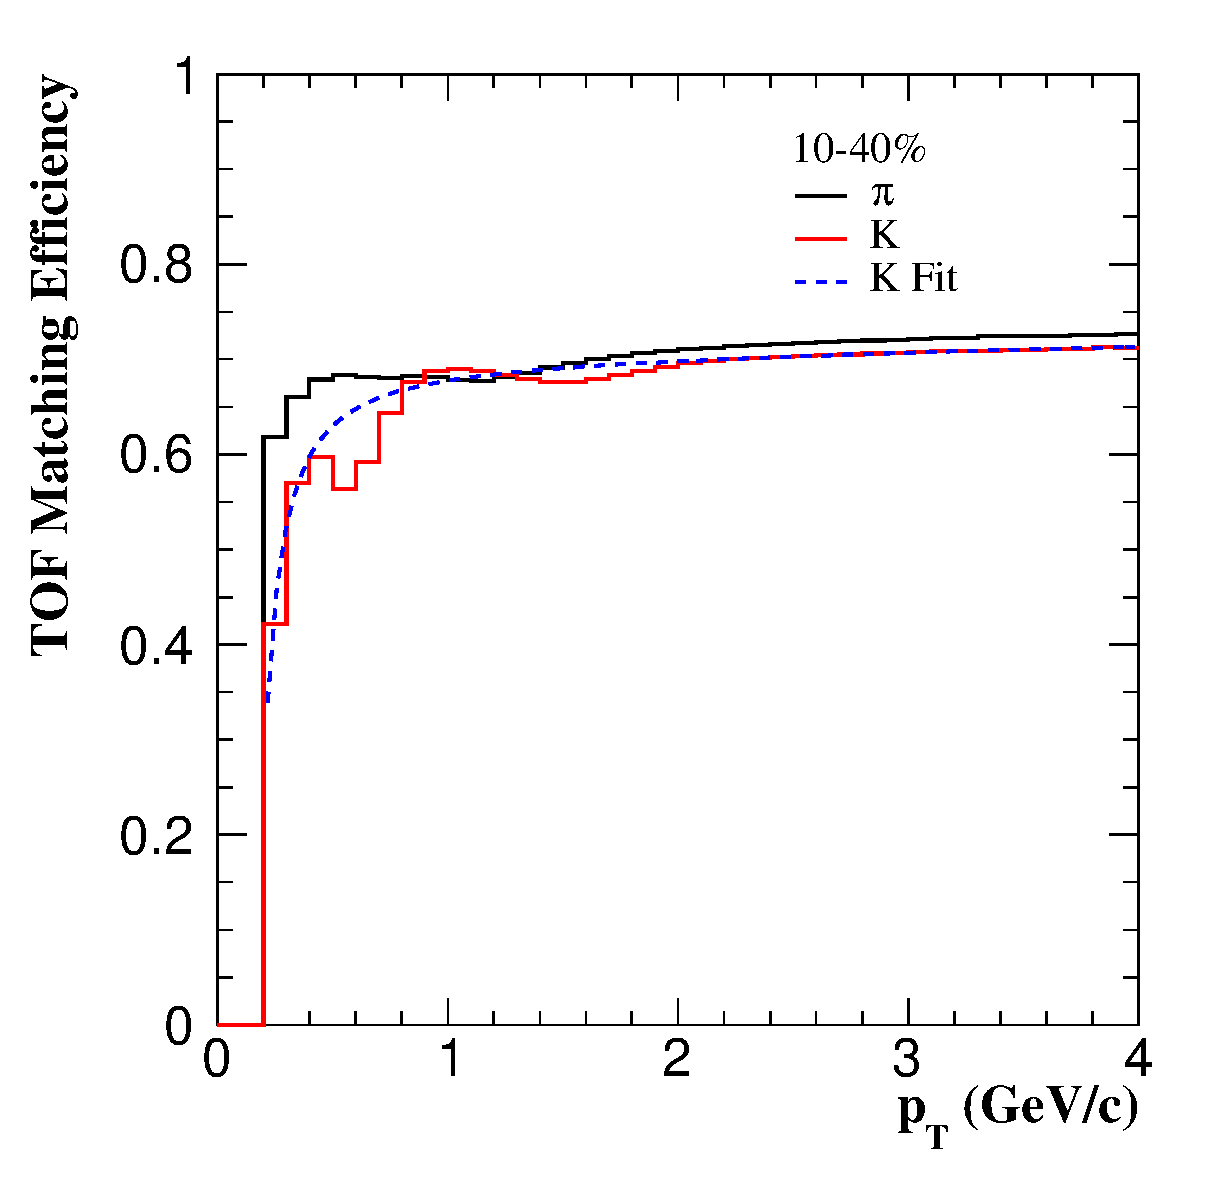
\includegraphics[width=0.47\textwidth]{{figure/Run11_xiaolong/efficiency/tofMatchRun11_10_40}.eps}}
    \subfigure{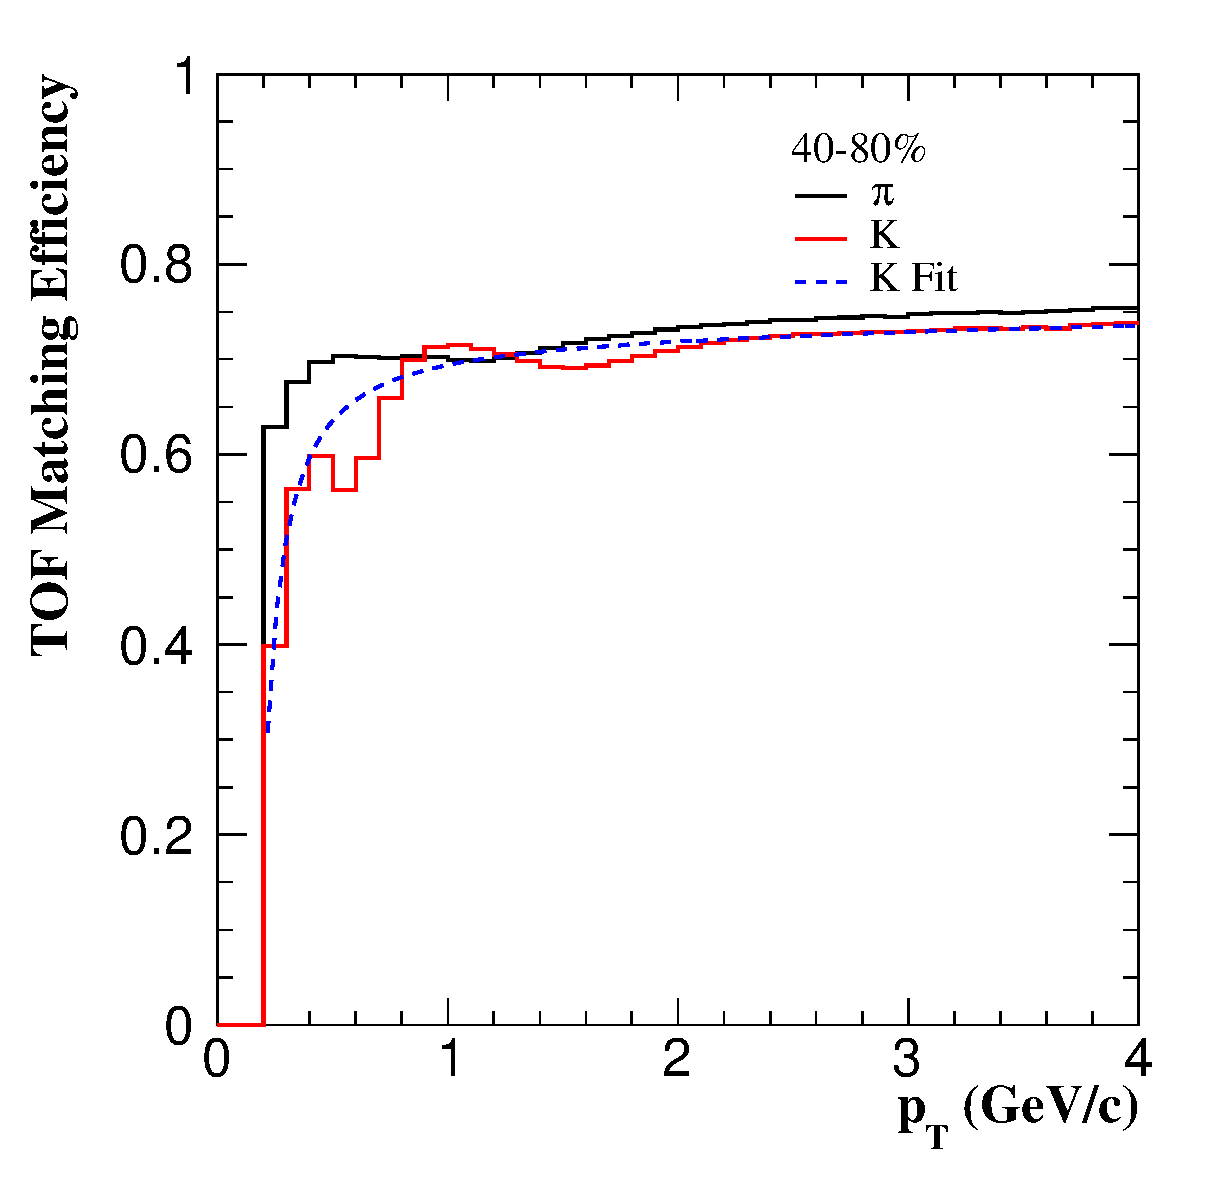
\includegraphics[width=0.47\textwidth]{{figure/Run11_xiaolong/efficiency/tofMatchRun11_40_80}.eps}}
    \caption{Run11 $K/\pi$ TOF matching efficiency at 0-80\%, 0-10\%, 10-40\%, 40-80\%.}
   \label{fig:Run11TofMatch}
\end{figure}

Fig.~\ref{fig:Run11singleEff} shows single cut efficiency.
\begin{figure}
    \centering
    \subfigure{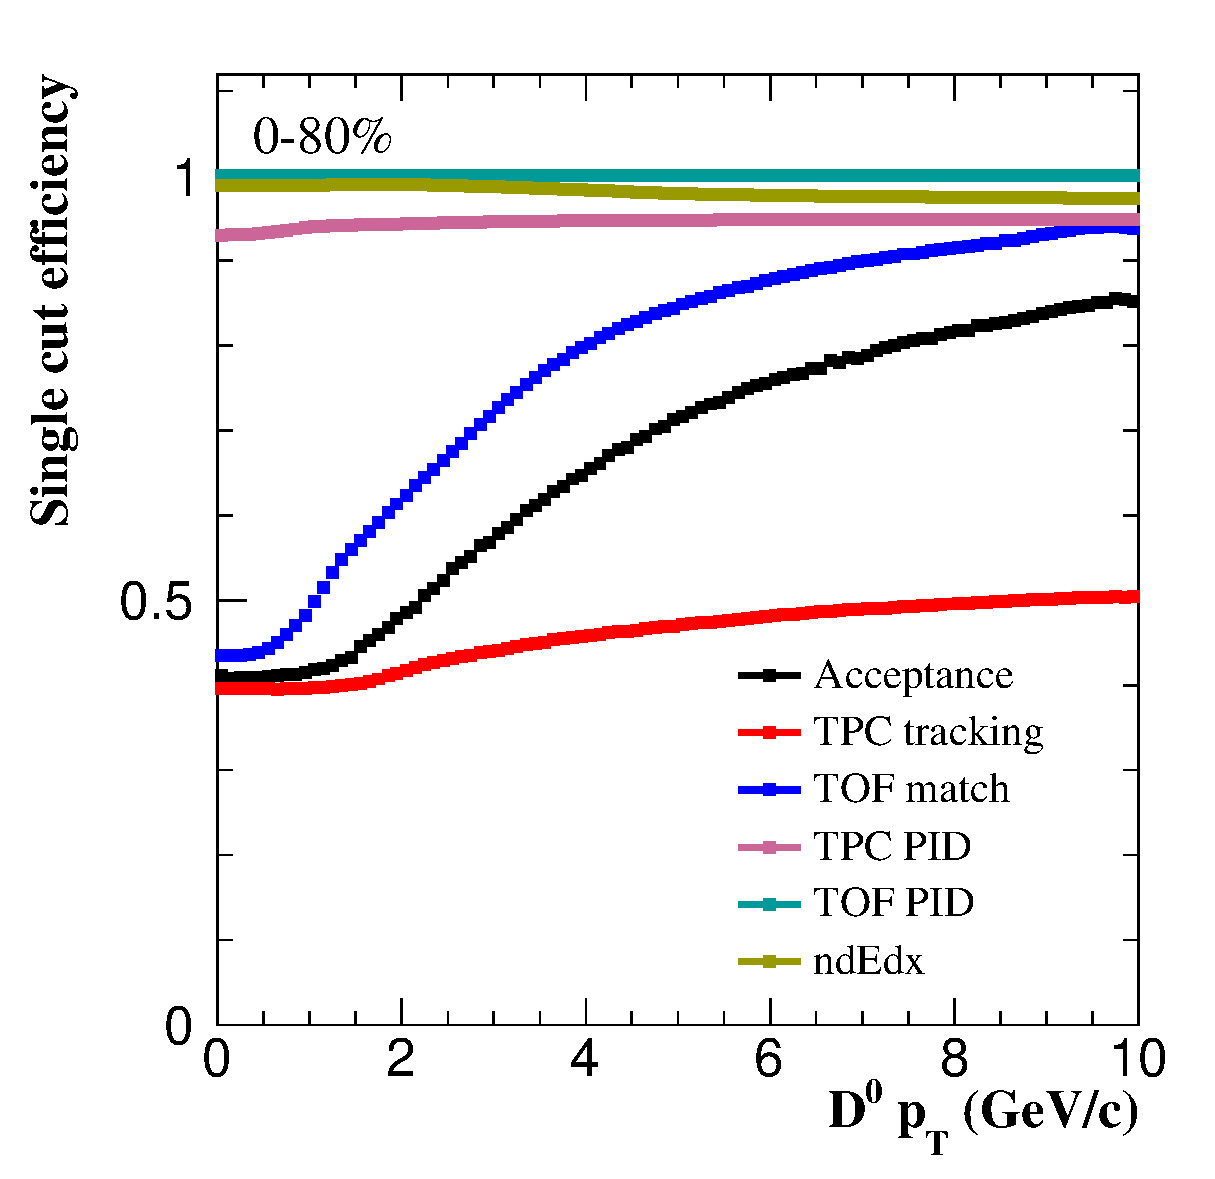
\includegraphics[width=0.5\textwidth]{{figure/Run11_xiaolong/efficiency/SingleCutEff}.eps}}
    \caption{Run11 single cut efficiency.}
   \label{fig:Run11singleEff}
\end{figure}

Fig.~\ref{fig:Run11D0eff} shows final $D^0$ efficiency in two PID cases, left panel for clean PID and right panel for hybrid PID.
\begin{figure}
    \centering
    \subfigure{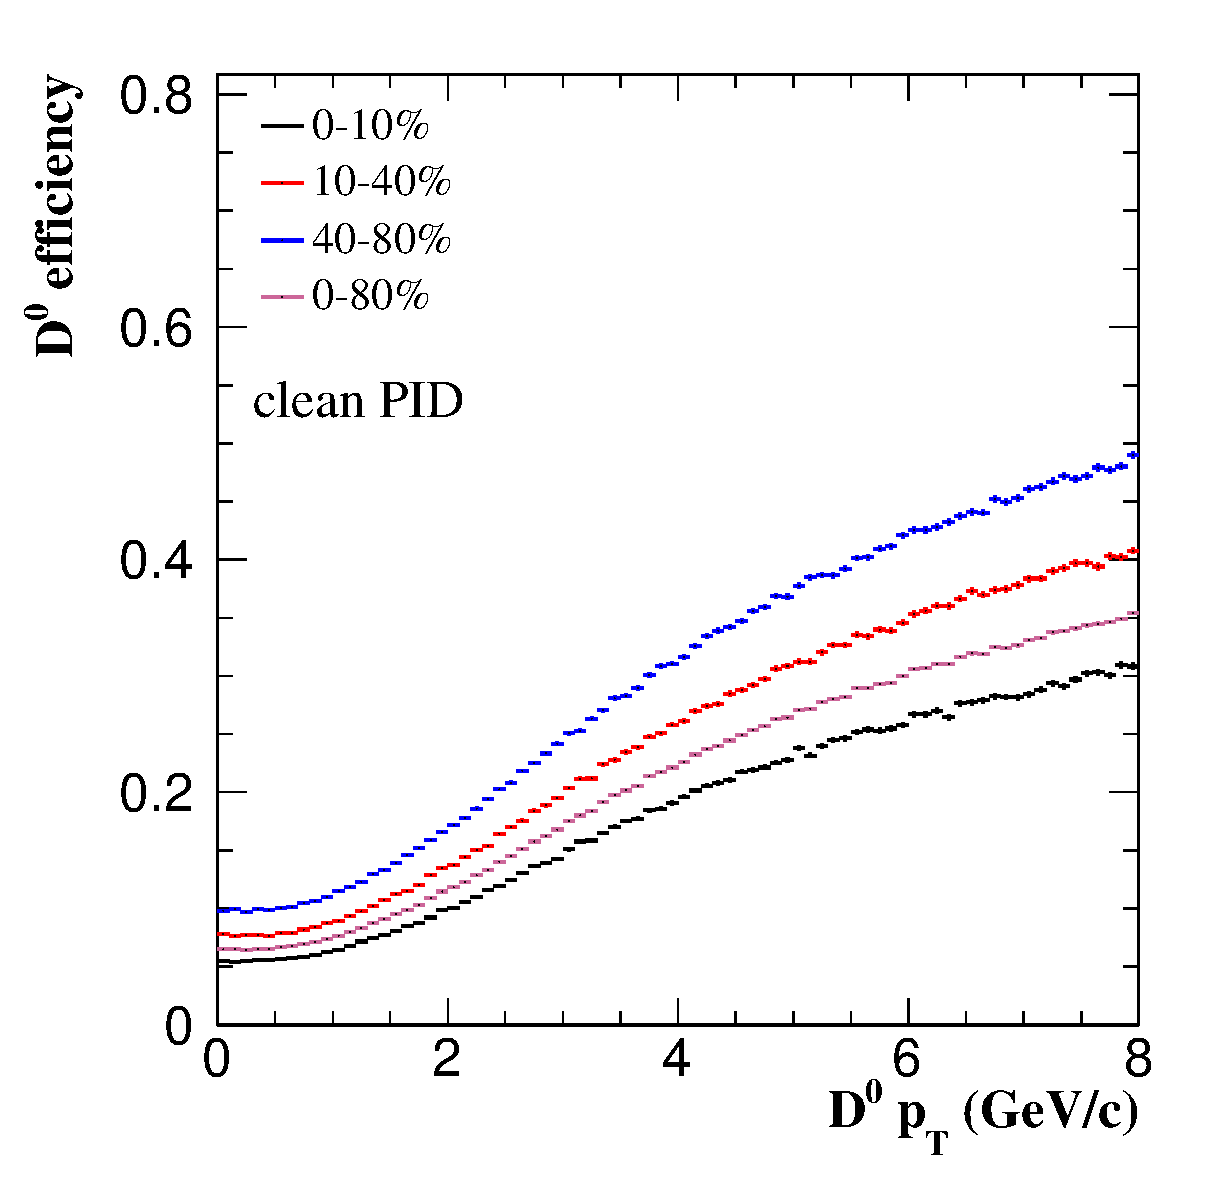
\includegraphics[width=0.47\textwidth]{{figure/Run11_xiaolong/efficiency/Run11_effAll_clean}.eps}}
    \subfigure{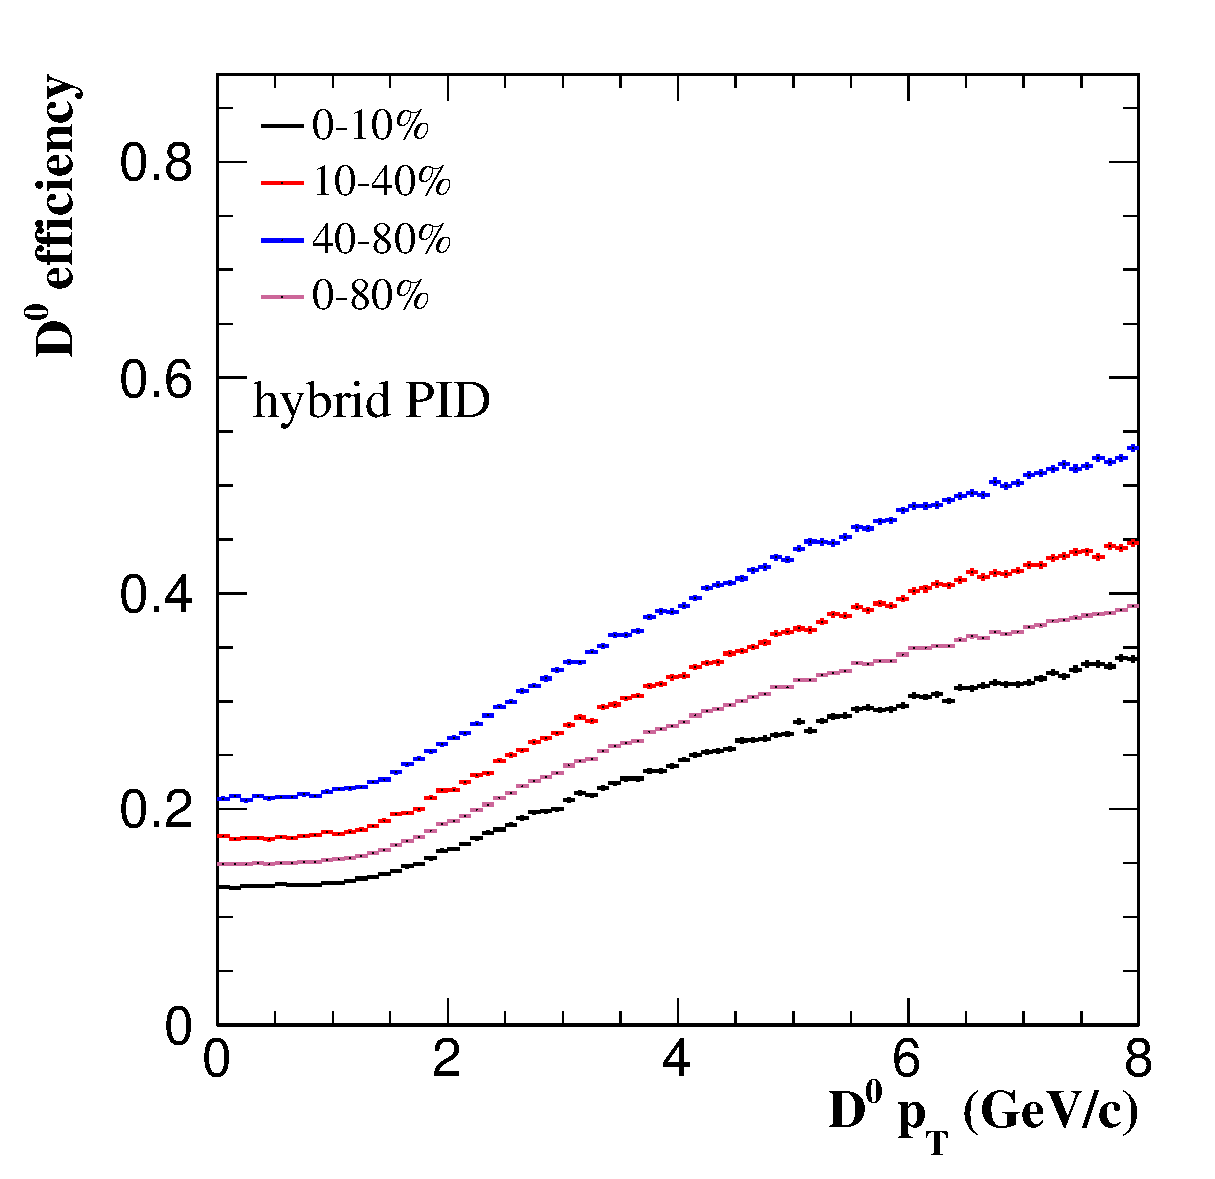
\includegraphics[width=0.47\textwidth]{{figure/Run11_xiaolong/efficiency/Run11_effAll_hybrid}.eps}}
    \caption{Run11 $D^0$ efficiency.}
   \label{fig:Run11D0eff}
\end{figure}

\subsubsection{Results}
Fig.~\ref{fig:Run11D0} shows $D^0$ spectra comparison between Run11 TPC and Run14 HFT in 6 $p_{T}$ bins. Top panel is $D^0$ spectra and bottom panel is the ratio of Run11 TPC over Run14 HFT. Those data points are removed in which $D^0$ significance is bad ($<$ 3) or $D^0$ width is too narrow ($<$ 9 MeV/$c^2$) or too wide ($>$ 25 MeV/$c^2$). Run11 TPC results are consistent with Run14 HFT results ($< 1\sigma$).
\begin{figure}
    \centering
    \subfigure{\includegraphics[width=0.5\textwidth]{{figure/Run11_xiaolong/ptDivision1/D0Run11_Spectra_0_80}.eps}}
    \caption{$D^0$ spectra comparison between Run11 TPC and Run14 HFT.}
   \label{fig:Run11D0}
\end{figure}

In order to get good $D^0$ significance in different centralities, we also use two wide $p_T$ bins (0-2 and 2-4 GeV/$c$).
Fig.~\ref{fig:Run11D0InCent} shows $D^0$ spectra comparison between Run11 TPC and Run14 HFT in two $p_{T}$ bins. In different centralities, Run11 TPC results are also consistent with Run14 HFT results ($< 1\sigma$).
\begin{figure}
    \centering
    \subfigure{\includegraphics[width=0.45\textwidth]{{figure/Run11_xiaolong/D0Run11_Spectra_0_80}.eps}}
    \subfigure{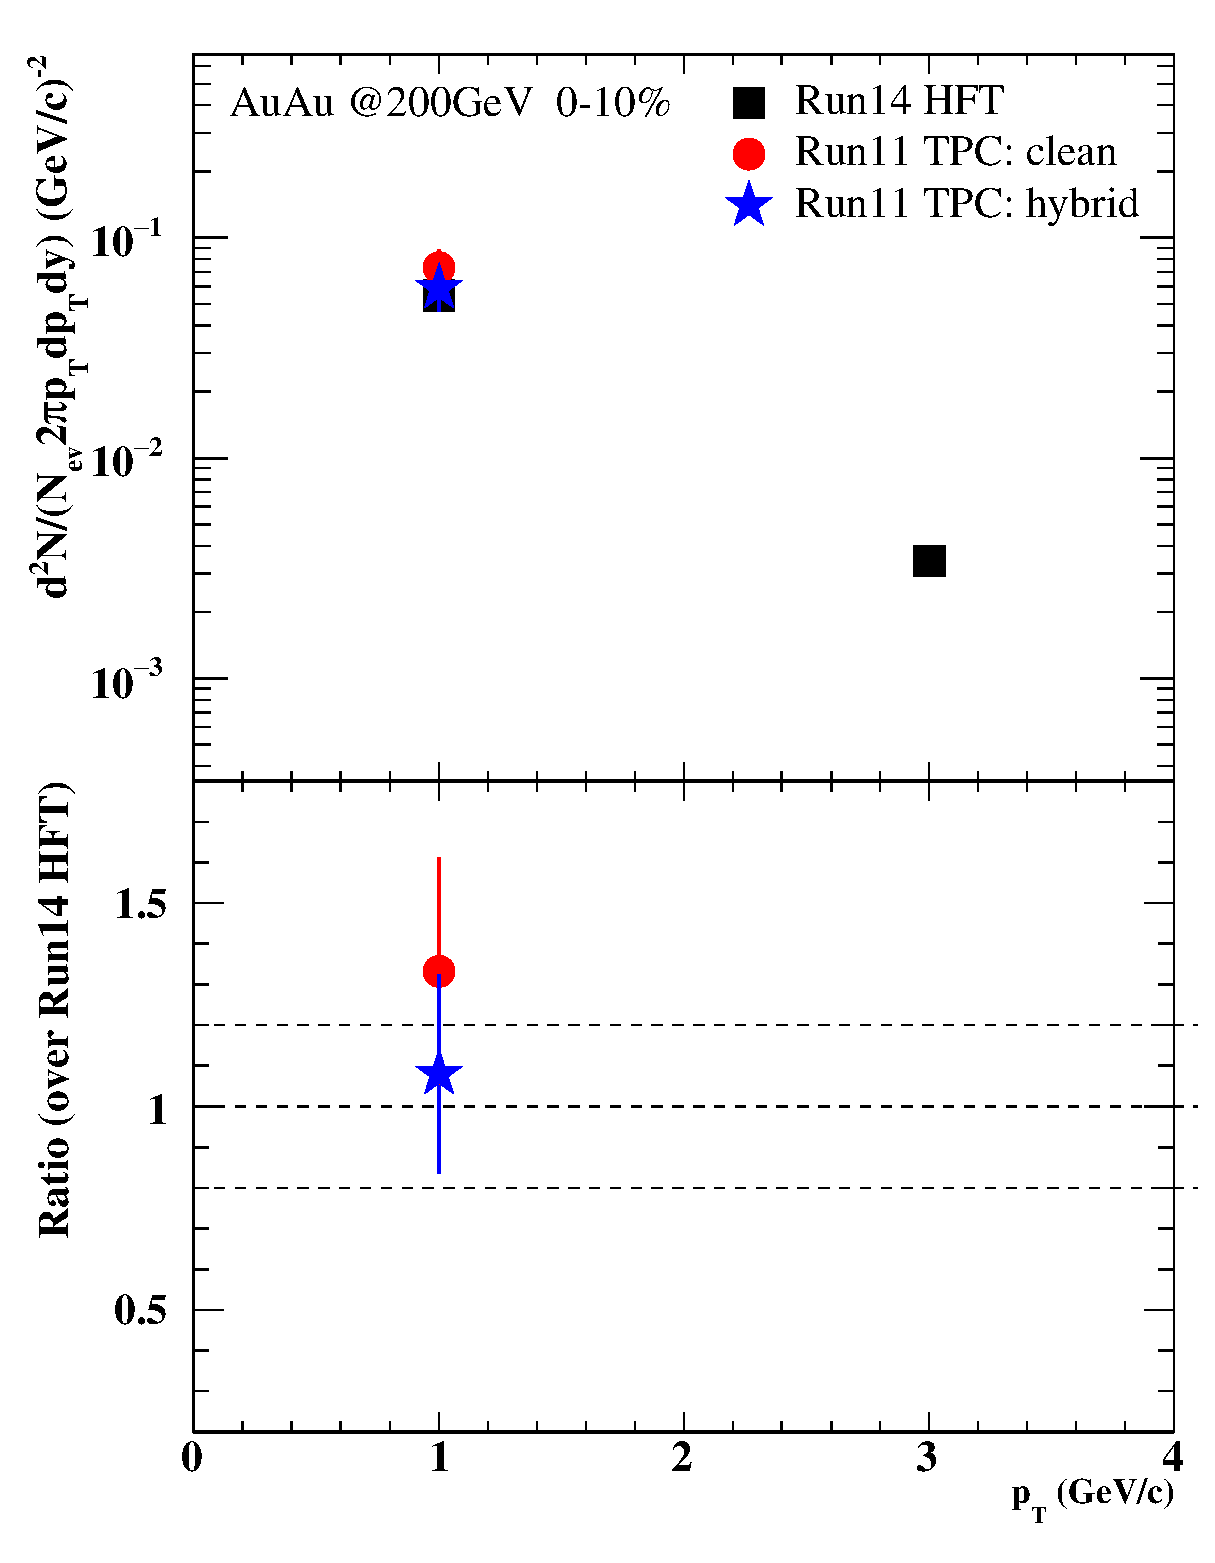
\includegraphics[width=0.45\textwidth]{{figure/Run11_xiaolong/D0Run11_Spectra_0_10}.eps}} \\
    \subfigure{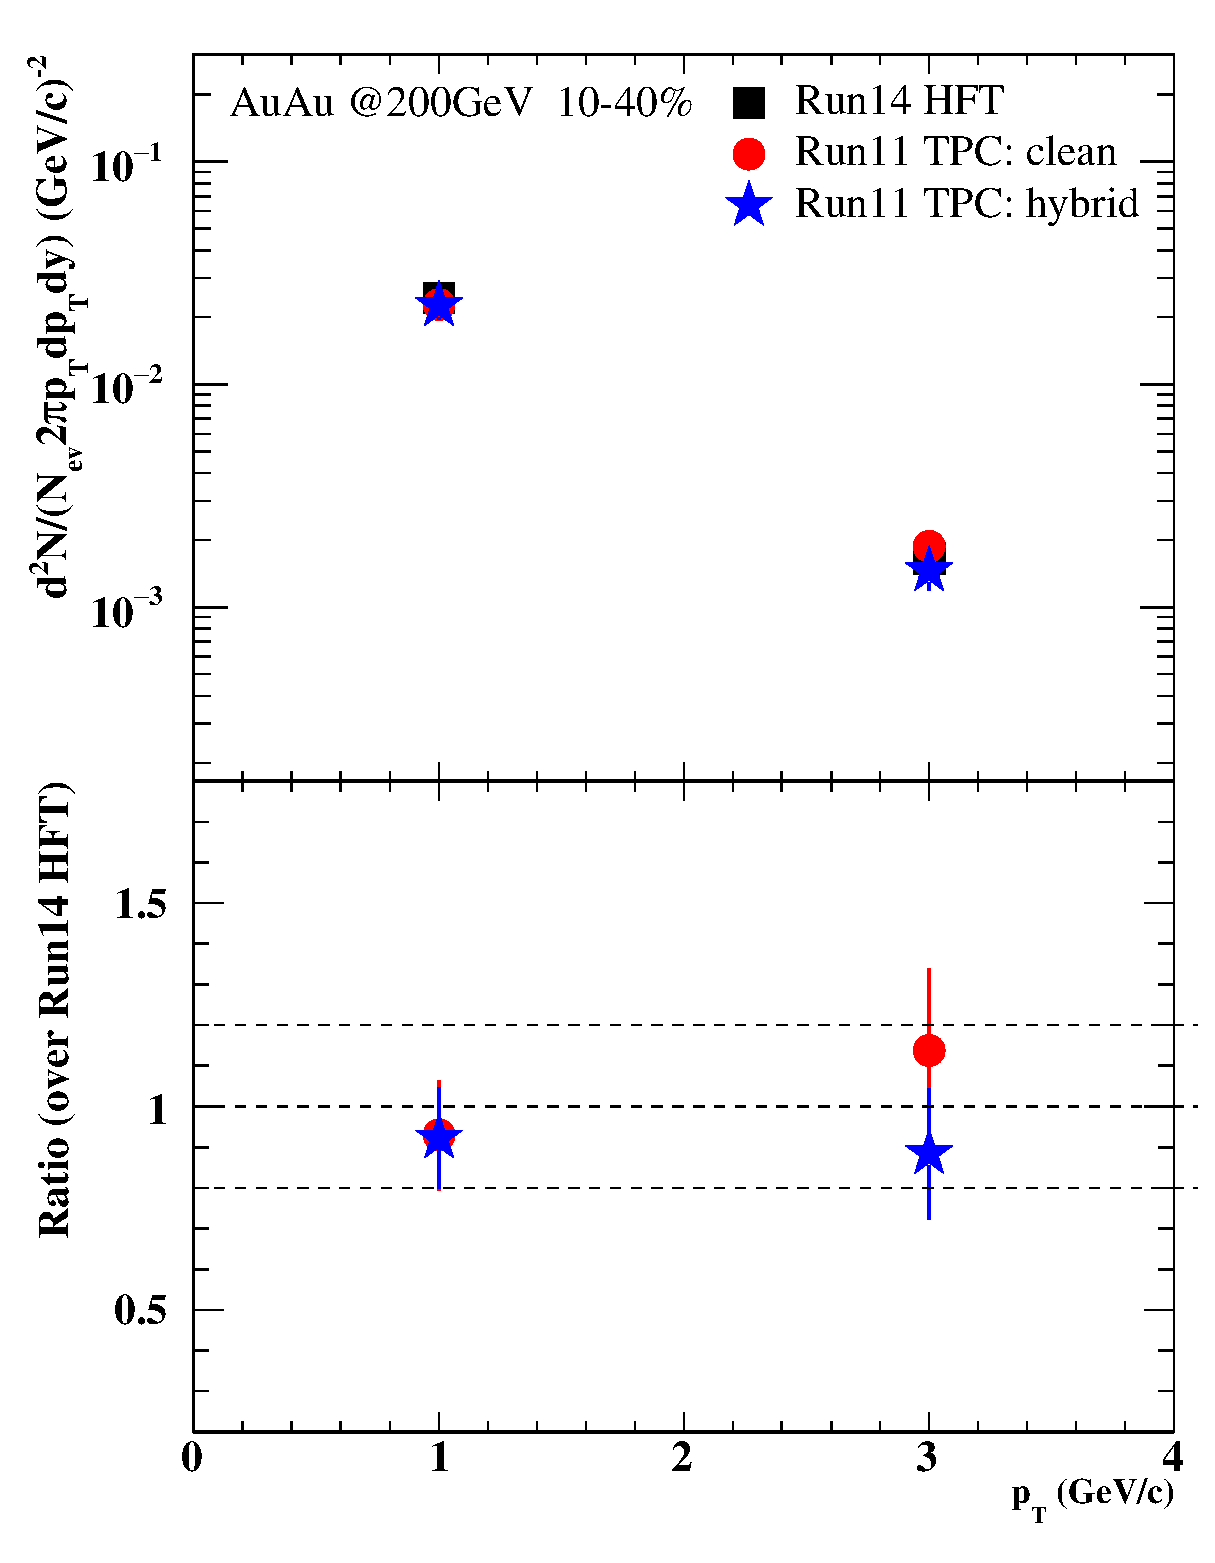
\includegraphics[width=0.45\textwidth]{{figure/Run11_xiaolong/D0Run11_Spectra_10_40}.eps}}
    \subfigure{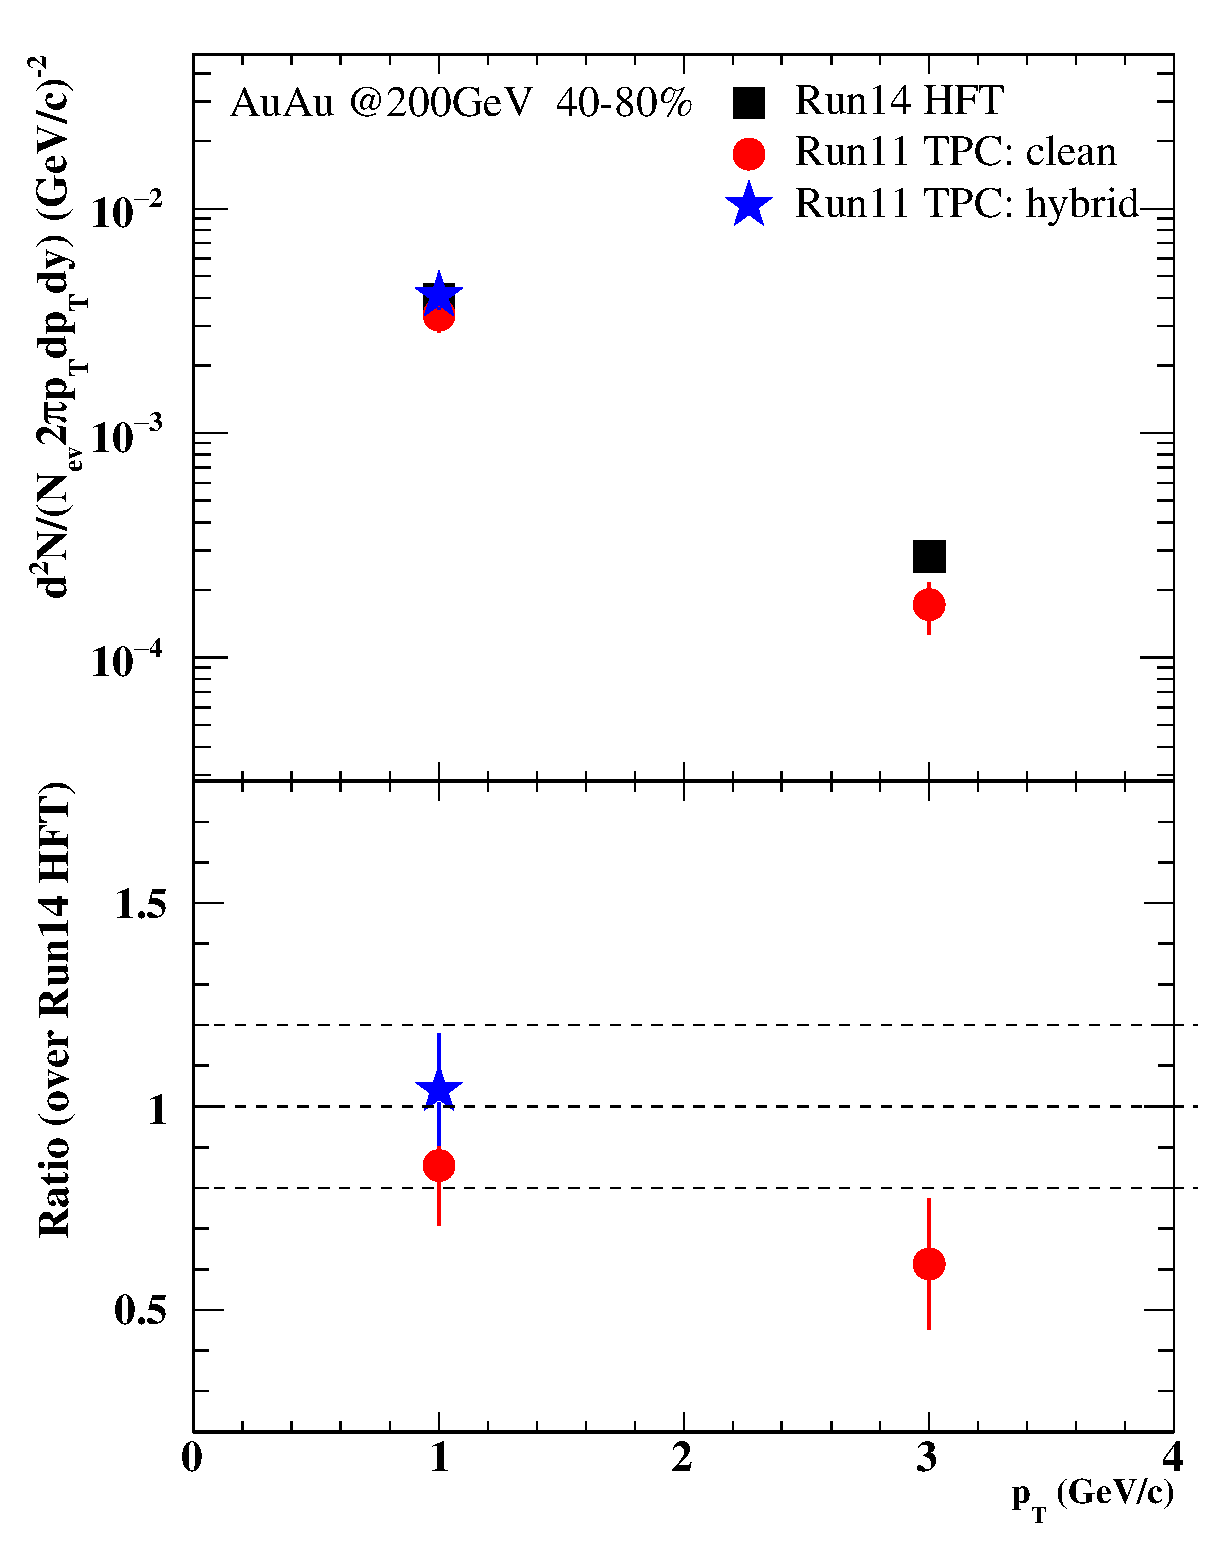
\includegraphics[width=0.45\textwidth]{{figure/Run11_xiaolong/D0Run11_Spectra_40_80}.eps}}
    \caption{$D^0$ spectra comparison between Run11 TPC and Run14 HFT in different centralities.}
   \label{fig:Run11D0InCent}
\end{figure}
